\documentclass{article}

\usepackage[a4paper, left=1.5cm, right=1.5cm, top=2cm, bottom=2cm]{geometry}
\usepackage{../../../../components/components}
\usepackage{hyperref}
\usepackage{fancyhdr}
\usepackage{amsfonts, amsmath, amssymb}

% Configuration des en-têtes et pieds de page
\pagestyle{fancy}
\fancyhf{}
\fancyhead[L]{DL$^\infty$ Math-Info}
\fancyhead[C]{Analyse}
\fancyhead[R]{2025-2026}
\fancyfoot[L]{Ewen Rodrigues de Oliveira}
\fancyfoot[R]{\thepage}

\begin{document}

\docTitle{Chapitre 11 : Fonctions de plusieurs variables}

\textbf{Cadre de travail :}
\begin{itemize}
    \item $p,q \in \mathbb{N}^*$
    \item $\mathcal{U}$ est un ouvert de $\mathbb{R}^q$
    \item $\mathbb{R}^p$ et $\mathbb{R}^q$ sont des espaces vectoriels qui peuvent être normés, donc des espaces métriques. Ainsi, toutes les propriétés et des notions des espaces métriques s'appliquent.
    \item $\| \cdot \|$ désigne une norme quelconque sur $\mathbb{R}^q$ ou $\mathbb{R}^p$ (les normes sont équivalentes en dimension finie, donc le choix de la norme n'affecte pas les propriétés étudiées).
\end{itemize}

\section{Continuité}

\definition{
    Soit $\mathcal{U}$ un ouvert de $\mathbb{R}^q$. Une fonction de plusieurs variables est définie par :
    \[ f : \mathcal{U} \to \mathbb{R}^p, \quad x \mapsto f(x) = f(x_1, \dots, x_q) \]
}

\example{
    Deux exemples de fonctions de plusieurs variables sont :
    \begin{enumerate}
        \item $f : \mathbb{R}^2 \to \mathbb{R}$, $(x,y) \mapsto x^2 + y^2$.
        \item $f : \mathbb{R}^3 \to \mathbb{R}^2$, $(x,y,z) \mapsto (x+y, yz)$.
    \end{enumerate}
}

\reminder{Une suite $(X_n)$ de composante $\begin{pmatrix}x^{(n)}_1 \\ x^{(n)}_2 \\ \vdots \\ x^{(n)}_p\end{pmatrix} \in \mathbb{R}^p$ tend vers $X = \begin{pmatrix}x_1 \\ x_2 \\ \vdots \\ x_p\end{pmatrix} \in \mathbb{R}^p$ si et seulement si chacune de ses composantes converge, c'est-à-dire :
\[
    \forall i \in \{1, \ldots, p\}, \quad x^{(n)}_i \xrightarrow[n \to +\infty]{} x_i
\]}
\definition{
    Soit $x_0 \in \mathcal{U}$ et soit $f : \mathcal{U} \to \mathbb{R}^p$.\\
    On dit que $f$ est continue en $x_0$ si :
    \[ \forall \epsilon > 0, \exists \alpha > 0, \forall x \in \mathcal{U}, \quad \|x - x_0\| \le \alpha \Rightarrow \|f(x) - f(x_0)\| < \epsilon \]
}

\theorem{Proposition}{Caractérisation de la continuité}{false}{
    Soit $f : \mathcal{U} \to \mathbb{R}^p$ et $x_0 \in \mathcal{U}$. Notons $f(x_0) = (f_1(x_0), \dots, f_p(x_0))$. Alors :
    \[
    f \text{ est continue en } x_0 \Leftrightarrow \forall i \in \{1, \dots, p\}, f_i \text{ est continue en } x_0
    \]
}

\noindent{\textbf{Preuve :}
\begin{itemize}
    \item $(\Rightarrow)$ : Supposons que $f$ est continue en $x_0$. Soit $i \in \{1, \dots, p\}$. Pour tout $\epsilon > 0$, il existe $\alpha > 0$ tel que pour tout $x \in \mathcal{U}$, $\|x - x_0\| \le \alpha$ implique $\|f(x) - f(x_0)\| < \epsilon$. En particulier, comme $|f_i(x) - f_i(x_0)| \le \|f(x) - f(x_0)\|$, on a bien $|f_i(x) - f_i(x_0)| < \epsilon$, donc $f_i$ est continue en $x_0$.
    \item $(\Leftarrow)$ : Supposons que pour tout $i \in \{1, \dots, p\}$, $f_i$ est continue en $x_0$. Soit $\epsilon > 0$. Pour chaque $i$, il existe $\alpha_i > 0$ tel que pour tout $x \in \mathcal{U}$, $\|x - x_0\| \le \alpha_i$ implique $|f_i(x) - f_i(x_0)| < \frac{\epsilon}{\sqrt{p}}$. Posons $\alpha = \min_{1 \le i \le p} \alpha_i$. Alors, pour tout $x \in \mathcal{U}$, $\|x - x_0\| \le \alpha$ implique que pour tout $i$, $|f_i(x) - f_i(x_0)| < \frac{\epsilon}{\sqrt{p}}$. Par conséquent :
    \[
    \|f(x) - f(x_0)\| = \sqrt{\sum_{i=1}^p (f_i(x) - f_i(x_0))^2} < \sqrt{p \cdot \left(\frac{\epsilon}{\sqrt{p}}\right)^2} = \epsilon
    \]
    Ainsi, $f$ est continue en $x_0$.
\end{itemize}
}

\remark{Par équivalence des normes en dimension finie, la notion de continuité ne dépend pas de la norme choisie dans $\mathbb{R}^q$.}

\attention{Il ne faut pas confondre les applications coordonnées et applications partielles : la continuité de toutes les applications partielles d'une fonction ne suffit pas à assurer sa continuité globale.}

\cexample{
    Soit $f(x,y) = \begin{cases} \frac{xy}{x^2+y^2} & \text{si } (x,y) \neq (0,0) \\ 0 & \text{sinon} \end{cases}$.\\
    Les applications partielles $x \mapsto f(x,0)$ et $y \mapsto f(0,y)$ sont nulles donc continues. Cependant, en approchant par la droite $y=x$ :
    \[ f(x,x) = \frac{x^2}{x^2+x^2} = \frac{1}{2} \xrightarrow[x \to 0]{} \frac{1}{2} \neq f(0,0) \]
    $f$ n'est pas continue en $(0,0)$.
}

\section{Dérivabilité et Différentiabilité}
\subsection{Dérivées partielles}

Soit $p, q \in \mathbb{N}^*$ et $\mathcal{U}$ un ouvert de $\mathbb{R}^p$. On considère une application $f : \mathcal{U} \to \mathbb{R}^q$.

\remark{Pour visualiser les concepts, on pourra penser au cas simple où $f : \mathbb{R}^2 \to \mathbb{R}$, dans lequel l'essentiel des propriétés et des difficultés de cette section se manifestent déjà.}

\subsubsection{Définition en un point et interprétation géométrique}
Soit $a = (a_1, \dots, a_p) \in \mathcal{U}$ et soit $k \in \{1, \dots, p\}$.

\definition{
    On appelle \textbf{$k$-ième fonction partielle} de $f$ au point $a$ l'application $g_k$ d'une variable réelle définie par :
    \[
    g_k : x_k \mapsto f(a_1, \dots, a_{k-1}, x_k, a_{k+1}, \dots, a_p)
    \]
    Cette fonction est définie sur un intervalle ouvert de $\mathbb{R}$ contenant $a_k$.
}

\definition{
    On dit que $f$ admet une \textbf{$k$-ième dérivée partielle} au point $a$ si la fonction partielle $g_k$ est dérivable au point $a_k$. 
    Le cas échéant, on note ce vecteur de $\mathbb{R}^q$ :
    \[
    \frac{\partial f}{\partial x_k}(a) = g_k'(a_k)
    \]
}

\theorem{Proposition}{Caractérisation de la dérivée partielle}{false}{
    L'existence de la $k$-ième dérivée partielle de $f$ en $a$ est équivalente à l'existence de la limite du taux d'accroissement suivant, où $e_k$ désigne le $k$-ième vecteur de la base canonique de $\mathbb{R}^p$ :
    \[
    \frac{\partial f}{\partial x_k}(a) = \lim_{t \to 0} \frac{f(a + t e_k) - f(a)}{t}
    \]
}

\subsubsection{Extension globale et pratique du calcul}

\definition{
    On dit que $f$ \textbf{admet des dérivées partielles} en $a$ si $\frac{\partial f}{\partial x_k}(a)$ existe pour tout $k \in \{1, \dots, p\}$ (autrement dit, si toutes ses dérivées partielles existent en ce point).
}
\vocabulary{On dit que $f$ admet des dérivées partielles sur $\mathcal{U}$ si elle admet des dérivées partielles en tout point de $\mathcal{U}$.}

\attention{
    Avant de calculer explicitement une dérivée partielle en un point par les règles usuelles, il est impératif de justifier son existence en vérifiant la dérivabilité de la fonction partielle correspondante.
}

\example{
    Soit $f : \mathbb{R}^2 \to \mathbb{R}$ définie par $f(x,y) = x^2 + y^2$. Soit $a = (a_1, a_2) \in \mathbb{R}^2$.
    \begin{itemize}
        \item Pour tout $y \in \mathbb{R}$ fixé, la fonction partielle $x \mapsto x^2 + y^2$ est polynomiale donc dérivable sur $\mathbb{R}$. Ainsi, la première dérivée partielle existe sur $\mathbb{R}^2$ et :
        \[ \frac{\partial f}{\partial x}(a_1, a_2) = 2a_1 \quad \text{notée usuellement} \quad \frac{\partial f}{\partial x}(x, y) = 2x \]
        \item Pour tout $x \in \mathbb{R}$ fixé, la fonction partielle $y \mapsto x^2 + y^2$ est également polynomiale donc dérivable sur $\mathbb{R}$. Ainsi, la seconde dérivée partielle existe sur $\mathbb{R}^2$ et :
        \[ \frac{\partial f}{\partial y}(a_1, a_2) = 2a_2 \quad \text{notée usuellement} \quad \frac{\partial f}{\partial y}(x, y) = 2y \]
    \end{itemize}
}

\subsubsection{Liens avec la continuité}
\attention{
    Contrairement aux fonctions d'une variable réelle, l'existence de toutes les dérivées partielles d'une fonction $f$ en un point $a$ \textbf{ne suffit pas} à garantir que $f$ soit continue en ce point.
}

\begin{figure}[htbp]
\centering
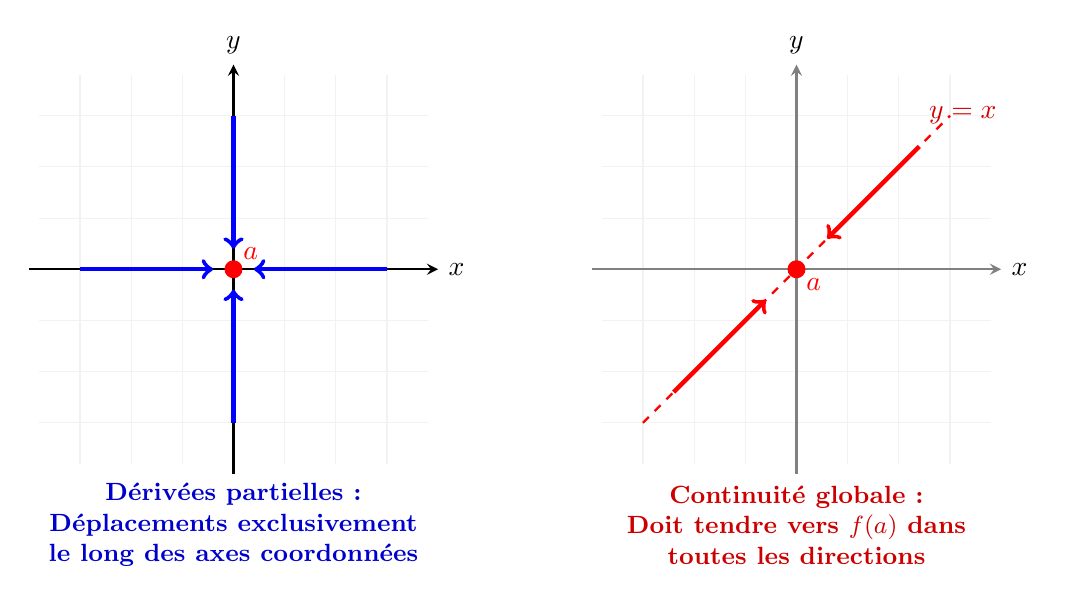
\begin{tikzpicture}[scale=1.3]

    % Premier volet : Dérivées partielles (déplacement le long des axes)
    \begin{scope}[shift={(0,0)}]
        % Grille d'arrière-plan légère
        \draw[gray!10, thin, step=0.5] (-1.9,-1.9) grid (1.9,1.9);
        
        % Axes
        \draw[->, >=stealth, thick] (-2,0) -- (2,0) node[right] {$x$};
        \draw[->, >=stealth, thick] (0,-2) -- (0,2) node[above] {$y$};
        
        % Flèches de déplacement le long des axes (bleues)
        \draw[blue, ultra thick, ->] (-1.5,0) -- (-0.2,0);
        \draw[blue, ultra thick, ->] (1.5,0) -- (0.2,0);
        \draw[blue, ultra thick, ->] (0,-1.5) -- (0,-0.2);
        \draw[blue, ultra thick, ->] (0,1.5) -- (0,0.2);
        
        % Point d'étude
        \fill[red] (0,0) circle (2.5pt);
        \node[red, above right] at (0,0) {$a$};
        
        \node[blue!80!black, font=\small\bfseries, align=center] at (0,-2.5) {Dérivées partielles :\\Déplacements exclusivement\\le long des axes coordonnées};
    \end{scope}

    % Second volet : Continuité (n'importe quelle direction, échec sur y = x)
    \begin{scope}[shift={(5.5,0)}]
        % Grille d'arrière-plan
        \draw[gray!10, thin, step=0.5] (-1.9,-1.9) grid (1.9,1.9);
        
        % Axes en gris pour atténuer
        \draw[->, >=stealth, gray, thick] (-2,0) -- (2,0) node[right, black] {$x$};
        \draw[->, >=stealth, gray, thick] (0,-2) -- (0,2) node[above, black] {$y$};
        
        % Droite y = x
        \draw[domain=-1.5:1.5, smooth, variable=\t, red, thick, dashed] plot ({\t},{\t});
        \node[red!80!black, right] at (1.2, 1.5) {$y=x$};
        
        % Approches directionnelles quelconques
        \draw[red, ultra thick, ->] (-1.2,-1.2) -- (-0.3,-0.3);
        \draw[red, ultra thick, ->] (1.2,1.2) -- (0.3,0.3);
        
        % Point d'étude
        \fill[red] (0,0) circle (2.5pt);
        \node[red, below right] at (0,0) {$a$};
        
        \node[red!80!black, font=\small\bfseries, align=center] at (0,-2.5) {Continuité globale :\\Doit tendre vers $f(a)$ dans\\toutes les directions};
    \end{scope}

\end{tikzpicture}
\caption{Visualisation de l'insuffisance des dérivées partielles pour la continuité en un point.}
\label{fig:continuite_vs_partielles}
\end{figure}
\cexample{
    Soit $f : \mathbb{R}^2 \to \mathbb{R}$ définie par :
    \[
    f(x,y) = \begin{cases} \frac{xy}{x^2 + y^2} & \text{si } (x,y) \neq (0,0) \\ 0 & \text{si } (x,y) = (0,0) \end{cases}
    \]
    \begin{enumerate}
        \item \textbf{Existence des dérivées partielles en $(0,0)$ :}
        \begin{itemize}
            \item La première fonction partielle en $(0,0)$ est $g_1(x) = f(x,0) = 0$ pour tout $x \in \mathbb{R}$. Cette fonction est nulle donc dérivable en $0$, d'où $\frac{\partial f}{\partial x}(0,0) = g_1'(0) = 0$.
            \item Par symétrie, la seconde fonction partielle en $(0,0)$ est $g_2(y) = f(0,y) = 0$. Elle est dérivable en $0$, d'où $\frac{\partial f}{\partial y}(0,0) = g_2'(0) = 0$.
        \end{itemize}
        Ainsi, $f$ admet des dérivées partielles en $(0,0)$ (et on montrerait de même qu'elles existent sur tout $\mathbb{R}^2$).
        
        \item \textbf{Défaut de continuité en $(0,0)$ :}
        Considérons la restriction de $f$ à la droite d'équation $y = x$. Pour tout $x \neq 0$ :
        \[
        f(x,x) = \frac{x^2}{x^2 + x^2} = \frac{1}{2}
        \]
        Par conséquent, $\lim_{x \to 0} f(x,x) = \frac{1}{2} \neq f(0,0)$. L'application $f$ n'est donc pas continue en $(0,0)$.
    \end{enumerate}
}

\noindent{\textit{Transition :} Le défaut de continuité observé dans le contre-exemple provient du fait que les dérivées partielles analysent uniquement le comportement de la fonction le long des axes de coordonnées. Dès que l'on s'approche de l'origine selon une autre trajectoire (comme la droite $y=x$), le comportement nous échappe. Cela motive l'introduction d'une notion plus générale s'affranchissant des axes du repère : la dérivée directionnelle.}

\subsection{Dérivées directionnelles}

Soit $f : \mathcal{U} \to \mathbb{R}^q$ où $\mathcal{U} \subset \mathbb{R}^p$ est un ouvert.
Soit $a \in \mathcal{U}$ et soit $h$ un vecteur de $\mathbb{R}^p$.
Considérons la fonction d'une variable réelle $\varphi : t \mapsto f(a + th)$ où $t$ varie dans un voisinage de $0$ tel que $a + th \in \mathcal{U}$.

\definition{
    On dit que $f$ admet une \textbf{dérivée directionnelle} en $a$ selon la direction (ou le vecteur) $h$ si la fonction $\varphi$ est dérivable en $0$. Le cas échéant, on note cette dérivée :
    \[
        D_h f(a) = \varphi'(0) = \lim_{t \to 0} \frac{f(a + th) - f(a)}{t}
    \]
}

% --- REPRÉSENTATION GÉOMÉTRIQUE AVEC TIKZ ---
\begin{figure}[htbp]
\centering
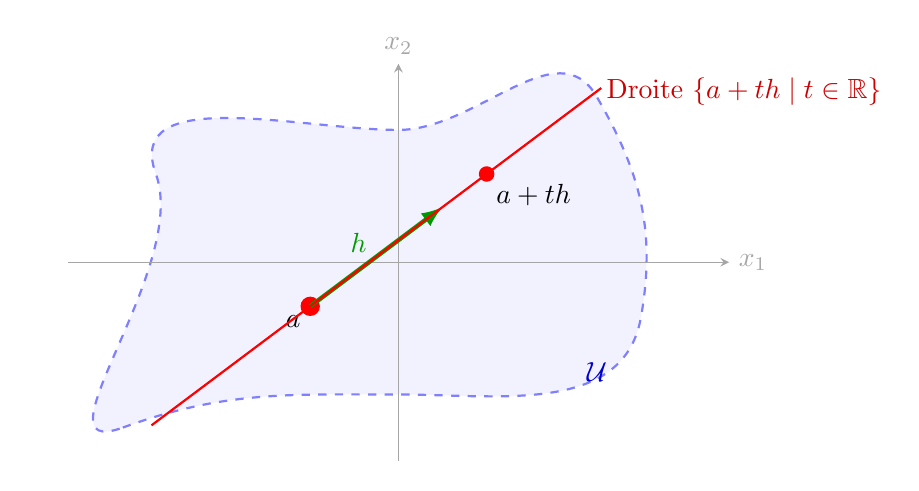
\begin{tikzpicture}[scale=1.4]
    % Dessin de l'ensemble U (forme ouverte et arrondie)
    \fill[blue!5, draw=blue!50, dashed, thick] 
        (-2.5,-1.5) to[out=20,in=180] (0,-1.2)
                    to[out=0,in=260] (2.2,-0.5)
                    to[out=80,in=300] (1.8,1.5)
                    to[out=120,in=0] (0,1.2)
                    to[out=180,in=110] (-2.2,0.8)
                    to[out=290,in=200] cycle;
    \node[blue!80!black] at (1.8,-1) {$\mathcal{U}$};

    % Axes de coordonnées discrets
    \draw[->, >=stealth, gray!70, thin] (-3,0) -- (3,0) node[right] {$x_1$};
    \draw[->, >=stealth, gray!70, thin] (0,-1.8) -- (0,1.8) node[above] {$x_2$};

    % Point a
    \coordinate (A) at (-0.8, -0.4);
    \fill[red] (A) circle (2.5pt) node[below left, black] {$a$};

    % Vecteur h
    \coordinate (H_end) at (0.4, 0.5); % vecteur (1.2, 0.9) relatif
    \draw[->, >=latex, green!60!black, ultra thick] (A) -- ++(1.2, 0.9) coordinate (B);
    \node[green!60!black, above left] at (-0.2, 0.0) {$h$};

    % Droite passant par a dirigée par h (représentée pour t réel)
    \draw[domain=-1.2:2.2, smooth, variable=\t, red, thick] plot ({ -0.8 + \t*1.2 }, { -0.4 + \t*0.9 });
    \node[red!80!black, right] at (1.8, 1.55) {Droite $\{a + th \mid t \in \mathbb{R}\}$};

    % Points de la forme a + th
    \coordinate (Ath) at (0.8, 0.8);
    \fill[red] (Ath) circle (2pt) node[below right, black] {$a + th$};
    
\end{tikzpicture}
\caption{Visualisation géométrique de l'étude locale dans la direction du vecteur $h$.}
\label{fig:directionnelle_geom}
\end{figure}

\theorem{Proposition}{Lien avec la dérivée partielle}{false}{
    Si on choisit comme direction $h = e_k$ (le $k$-ième vecteur de la base canonique de $\mathbb{R}^p$), alors la dérivée directionnelle de $f$ en $a$ selon la direction $e_k$ est la $k$-ième dérivée partielle de $f$ en $a$.
}

\noindent{\textbf{Preuve :}}\\
En posant $h = e_k$, la fonction de l'évaluation locale s'écrit pour $t$ proche de 0 :
\[
\varphi(t) = f(a + te_k) = f(a_1, \ldots, a_{k-1}, a_k + t, a_{k+1}, \ldots, a_p)
\]
On observe alors que $\varphi(t) = g_k(a_k + t)$ où $g_k$ est la $k$-ième fonction partielle définie dans la section précédente.
Par conséquent, la dérivabilité de $\varphi$ en $0$ équivaut précisément à la dérivabilité de la fonction partielle $g_k$ en $a_k$. On en conclut que :
\[
D_{e_k} f(a) = \varphi'(0) = g_k'(a_k) = \frac{\partial f}{\partial x_k}(a)
\]
\hfill $\square$

\example{
    Étudions la dérivée directionnelle en toutes les directions au point $a = (0,0)$ de la fonction $f$ définie sur $\mathbb{R}^2$ par :
    \[
    f(x,y) = \begin{cases} \frac{xy}{x^2 + y^2} & \text{si } (x,y) \neq (0,0) \\ 0 & \text{si } (x,y) = (0,0) \end{cases}
    \]
    
    \noindent Soit $h = (h_1, h_2) \in \mathbb{R}^2$ un vecteur non nul représentatif de la direction choisie. Par définition, on cherche à étudier la dérivabilité en $t=0$ de la fonction d'une variable réelle :
    \[
    \varphi : t \mapsto f(a + th) = f(th) = f(th_1, th_2)
    \]
    Pour tout $t \neq 0$, le point $(th_1, th_2)$ est distinct de $(0,0)$. On a donc :
    \[
    \varphi(t) = \frac{(th_1)(th_2)}{(th_1)^2 + (th_2)^2} = \frac{t^2 h_1 h_2}{t^2 (h_1^2 + h_2^2)} = \frac{h_1 h_2}{h_1^2 + h_2^2}
    \]
    On calcule maintenant la limite du taux d'accroissement de $\varphi$ en $0$ lorsque $t \to 0$ :
    \[
    \frac{\varphi(t) - \varphi(0)}{t} = \frac{\frac{h_1 h_2}{h_1^2 + h_2^2} - 0}{t} = \frac{1}{t} \cdot \frac{h_1 h_2}{h_1^2 + h_2^2}
    \]
    Distinguons alors deux cas selon la direction du vecteur $h$ :
    \begin{itemize}
        \item \textbf{Cas 1 : } Si $h_1 = 0$ ou $h_2 = 0$ (déplacement le long de l'axe des abscisses ou des ordonnées). \\
        Le numérateur $h_1 h_2$ est nul. Le taux d'accroissement est identiquement nul pour tout $t \neq 0$, sa limite en $0$ existe et vaut $0$. Ainsi, les dérivées directionnelles selon les axes de coordonnées existent et l'on retrouve les dérivées partielles : $D_{(1,0)}f(0,0) = 0$ et $D_{(0,1)}f(0,0) = 0$.
        
        \item \textbf{Cas 2 : } Si $h_1 \neq 0$ et $h_2 \neq 0$ (déplacement hors des axes). \\
        La quantité $\frac{h_1 h_2}{h_1^2 + h_2^2}$ est une constante réelle non nulle. Par conséquent :
        \[
        \lim_{t \to 0^{\pm}} \frac{1}{t} \cdot \frac{h_1 h_2}{h_1^2 + h_2^2} = \pm \infty
        \]
        La limite n'étant pas finie, la fonction $\varphi$ n'est pas dérivable en $0$.
    \end{itemize}
    \textbf{Conclusion : } La fonction $f$ admet des dérivées directionnelles en $(0,0)$ uniquement selon les directions des axes de coordonnées (les dérivées partielles). Elle n'en admet dans aucune autre direction.
}

\attention{
    L'existence de toutes les dérivées directionnelles d'une fonction $f$ en un point $a$ \textbf{ne suffit toujours pas} à garantir sa continuité en ce point.
}

\training{
Considérer la fonction $f : \mathbb{R}^2 \to \mathbb{R}$ définie par :
\[
f(x,y)=\begin{cases} \frac{y^2}{x} & \text{si } x \neq 0 \\ y & \text{sinon} \end{cases}
\]
\begin{enumerate}
    \item Montrer que $f$ admet des dérivées directionnelles en tout point de $\mathbb{R}^2$ et dans toutes les directions.
    \item Montrer que $f$ n'est pas continue en $(0,1)$ (on pourra s'intéresser à la suite de points $(\frac{1}{n},1)$).
\end{enumerate}
}
\noindent\carreaux{13}
\subsection{La notion de différentiabilité}

La différentiabilité est la véritable extension de la notion de dérivabilité aux espaces de plusieurs variables. Contrairement aux dérivées partielles ou directionnelles, elle assure une approximation linéaire globale de la fonction au voisinage d'un point.

Dans toute cette section, $\mathcal{U}$ désigne un ouvert de $\mathbb{R}^p$.

\subsubsection{Définition générale}

\definition{
    Soit $f : \mathcal{U} \to \mathbb{R}^q$ et $a \in \mathcal{U}$. On dit que $f$ est \textbf{différentiable} au point $a$ s'il existe une application linéaire $L \in \mathcal{L}(\mathbb{R}^p, \mathbb{R}^q)$ telle que, pour tout $h \in \mathbb{R}^p$ tel que $a+h \in \mathcal{U}$ :
    \[
    f(a+h) = f(a) + L(h) + o(\|h\|) \quad \text{quand } h \to 0
    \]
    c'est-à-dire $f(a+h) = f(a) + L(h) + \|h\|\varepsilon(h)$ avec $\lim_{h \to 0} \varepsilon(h) = 0_{\mathbb{R}^q}$.\\
    Si une telle application linéaire existe, elle est unique. On l'appelle la \textbf{différentielle} de $f$ en $a$ et on la note $Df(a)$.
}

\example{
    Soit $f : \mathbb{R} \to \mathbb{R}$ une fonction d'une variable réelle dérivable en $a$. La formule de Taylor-Young donne $f(a+h) = f(a) + f'(a)h + o(h)$. La différentielle $Df(a)$ est l'application linéaire de $\mathcal{L}(\mathbb{R}, \mathbb{R})$ définie par :
    \[ Df(a) : h \mapsto f'(a) \cdot h \]
    Il s'agit géométriquement de l'application linéaire associée à la multiplication par le scalaire $f'(a)$.
}

\example{
    Soit $f \in \mathcal{L}(\mathbb{R}^p, \mathbb{R}^q)$ une application linéaire. Pour tout $a \in \mathbb{R}^p$ et tout $h \in \mathbb{R}^p$, on a par linéarité :
    \[ f(a+h) = f(a) + f(h) + 0 \]
    Le reste étant identiquement nul, il est un $o(\|h\|)$. Ainsi, $f$ est différentiable en tout point $a \in \mathbb{R}^p$ et sa différentielle est l'application $f$ elle-même, indépendamment du point $a$ :
    \[ \forall a \in \mathbb{R}^p, \quad Df(a) = f \]
}

\subsubsection{Propriétés fondamentales}

Le premier grand intérêt de la différentiabilité est qu'elle résout les défauts des notions précédentes en garantissant la continuité.

\theorem{Proposition}{Différentiabilité implique continuité}{false}{
    Si $f : \mathcal{U} \to \mathbb{R}^q$ est différentiable en $a \in \mathcal{U}$, alors $f$ est continue en $a$.
}

\noindent{\textbf{Preuve :}\\
Soit $f$ différentiable en $a$. Pour tout $h$ au voisinage de $0$, on a par l'inégalité triangulaire :
\[ \|f(a+h) - f(a)\| \leq \|Df(a) \cdot h\| + \|o(\|h\|)\| \]
Puisque nous sommes en dimension finie, l'application linéaire $Df(a)$ est automatiquement continue. Il existe donc une constante $C_a > 0$ telle que $\|Df(a) \cdot h\| \leq C_a \|h\|$. On en déduit :
\[ \|f(a+h) - f(a)\| \leq C_a \|h\| + \|h\|\|\varepsilon(h)\| = \|h\| \big(C_a + \|\varepsilon(h)\|\big) \]
Lorsque $h \to 0$, le membre de droite tend vers $0$. On a donc $\lim_{h \to 0} f(a+h) = f(a)$, ce qui prouve la continuité de $f$ en $a$. \hfill $\square$
}

\theorem{Proposition}{Lien avec les dérivées directionnelles}{false}{
    Si $f : \mathcal{U} \to \mathbb{R}^q$ est différentiable en $a \in \mathcal{U}$, alors $f$ admet des dérivées directionnelles en $a$ selon toutes les directions $h \in \mathbb{R}^p$, et on a :
    \[ Df(a) \cdot h = \lim_{t \to 0} \frac{f(a+th) - f(a)}{t} \]
}

\noindent{\textbf{Preuve :}\\
Soit $h \in \mathbb{R}^p$. En évaluant le développement limité de $f$ en $a$ le long de la droite passant par $a$ et de vecteur directeur $h$ (pour $t \in \mathbb{R}$ proche de $0$), on obtient par linéarité de $Df(a)$ :
\[ f(a+th) = f(a) + Df(a) \cdot (th) + o(\|th\|) = f(a) + t \big(Df(a) \cdot h\big) + |t|\|h\|\varepsilon(th) \]
Formons le taux d'accroissement pour $t \neq 0$ :
\[ \frac{f(a+th) - f(a)}{t} = Df(a) \cdot h + \frac{|t|}{t} \|h\|\varepsilon(th) \]
Puisque $\lim_{t \to 0} \varepsilon(th) = 0$ et que le facteur $\frac{|t|}{t}$ est borné (il vaut $\pm 1$), le second terme tend vers $0_{\mathbb{R}^q}$ quand $t \to 0$. On obtient bien :
\[ \lim_{t \to 0} \frac{f(a+th) - f(a)}{t} = Df(a) \cdot h \]
L'application $t \mapsto f(a+th)$ est donc dérivable en $0$, ce qui prouve l'existence de la dérivée directionnelle, égale à $Df(a) \cdot h$. \hfill $\square$
}

\remark{La réciproque est fausse. Une fonction peut admettre des dérivées directionnelles dans toutes les directions sans pour autant être différentiable.}

\cexample{
    Considérons une norme quelconque $\|\cdot\| : \mathbb{R}^p \to \mathbb{R}$. Montrons que cette fonction n'est pas différentiable en $a = 0_{\mathbb{R}^p}$.\\
    Pour tout vecteur non nul $h \in \mathbb{R}^p$ et tout $t \in \mathbb{R}^*$, le taux d'accroissement en $0$ s'écrit :
    \[ \frac{\|0 + th\| - \|0\|}{t} = \frac{|t|\|h\|}{t} = \frac{|t|}{t}\|h\| \]
    Cette quantité admet pour limites à droite et à gauche en $0$ respectivement $+\|h\|$ et $-\|h\|$. La limite n'existe pas en $0$ car $h \neq 0_{\mathbb{R}^p}$. La fonction norme n'admet donc pas de dérivées directionnelles à l'origine, elle n'y est donc pas différentiable.
}

\subsubsection{Cas des fonctions scalaires : Le Gradient}

Lorsque l'espace d'arrivée est $\mathbb{R}$ ($q=1$), la différentielle $Df(a)$ est une forme linéaire ($\in \mathcal{L}(\mathbb{R}^p, \mathbb{R})$). Le théorème de représentation de Riesz permet de l'identifier à un vecteur via le produit scalaire usuel, noté $\langle \cdot, \cdot \rangle$.

\theorem{Proposition et définition}{Le Gradient}{false}{
    Soit $f : \mathcal{U} \to \mathbb{R}$ une fonction différentiable en $a \in \mathcal{U}$. Il existe un unique vecteur de $\mathbb{R}^p$, appelé \textbf{gradient} de $f$ en $a$ et noté $\nabla f(a)$, tel que :
    \[ \forall h \in \mathbb{R}^p, \quad Df(a) \cdot h = \langle \nabla f(a), h \rangle \]
    Dans la base canonique de $\mathbb{R}^p$, ce vecteur a pour coordonnées les dérivées partielles de $f$ :
    \[ \nabla f(a) = \begin{pmatrix} \frac{\partial f}{\partial x_1}(a) \\ \vdots \\ \frac{\partial f}{\partial x_p}(a) \end{pmatrix} \]
}

\noindent{\textbf{Preuve :}\\
Soit $(e_1, \dots, e_p)$ la base canonique de $\mathbb{R}^p$. Pour tout $h = \sum_{i=1}^p h_i e_i \in \mathbb{R}^p$, on a par linéarité de la différentielle :
\[ Df(a) \cdot h = Df(a) \cdot \left(\sum_{i=1}^p h_i e_i\right) = \sum_{i=1}^p h_i \big(Df(a) \cdot e_i\big) \]
Or, d'après les liens avec les dérivées directionnelles et partielles, $Df(a) \cdot e_i = \frac{\partial f}{\partial x_i}(a)$. Ainsi :
\[ Df(a) \cdot h = \sum_{i=1}^p \frac{\partial f}{\partial x_i}(a) h_i \]
Cette expression correspond exactement au produit scalaire usuel $\langle \nabla f(a), h \rangle$ en posant pour $\nabla f(a)$ le vecteur colonne des dérivées partielles. \hfill $\square$
}

\definition{
    Soit $f : \mathcal{U} \to \mathbb{R}$ une fonction différentiable. On appelle \textbf{point critique} de $f$ tout point $x \in \mathcal{U}$ où le gradient s'annule, c'est-à-dire :
    \[ \nabla f(x) = 0_{\mathbb{R}^p} \]
}

\example{
    Soit $f(x,y,z) = x^2 (1 + z \cos(y))$ définie sur $\mathbb{R}^3$. Son gradient est donné par :
    \[ \nabla f(x,y,z) = \begin{pmatrix} 2x(1 + z \cos(y)) \\ -x^2 z \sin(y) \\ x^2 \cos(y) \end{pmatrix} \]
    Calculons la dérivée directionnelle de $f$ au point $a = (1,\pi,1)$ selon le vecteur $h = (1,1,1)^T$. On évalue d'abord le gradient en $a$ :
    \[ \nabla f(1,\pi,1) = \begin{pmatrix} 2(1) (1 + 1 \cdot \cos(\pi)) \\ -1^2 \cdot 1 \cdot \sin(\pi) \\ 1^2 \cos(\pi) \end{pmatrix} = \begin{pmatrix} 2(1-1) \\ 0 \\ -1 \end{pmatrix} = \begin{pmatrix} 0 \\ 0 \\ -1 \end{pmatrix} \]
    La dérivée directionnelle cherchée vaut alors :
    \[ Df(1,\pi,1) \cdot h = \langle \nabla f(1,\pi,1), h \rangle = \left\langle \begin{pmatrix} 0 \\ 0 \\ -1 \end{pmatrix} , \begin{pmatrix} 1 \\ 1 \\ 1 \end{pmatrix} \right\rangle = 0\cdot 1 + 0\cdot 1 + (-1)\cdot 1 = -1 \]
}

\subsubsection{Cas des fonctions vectorielles : La Matrice Jacobienne}

Lorsque $f : \mathcal{U} \to \mathbb{R}^q$, la différentielle $Df(a)$ est représentée matriciellement dans les bases canoniques de $\mathbb{R}^p$ et $\mathbb{R}^q$.

\definition{
    Soit $f : \mathcal{U} \to \mathbb{R}^q$ une fonction différentiable en $a \in \mathcal{U}$. On appelle \textbf{matrice jacobienne} de $f$ en $a$, notée $J_f(a)$, la matrice de l'application linéaire $Df(a)$ exprimée dans les bases canoniques de départ et d'arrivée.\\
    Cette matrice appartient à $\mathcal{M}_{q,p}(\mathbb{R})$ et ses coefficients sont donnés par les dérivées partielles des composantes $f_i$ de $f$ :
    \[
    J_f(a) = \begin{pmatrix}
        \frac{\partial f_1}{\partial x_1}(a) & \frac{\partial f_1}{\partial x_2}(a) & \ldots & \frac{\partial f_1}{\partial x_p}(a) \\
        \frac{\partial f_2}{\partial x_1}(a) & \frac{\partial f_2}{\partial x_2}(a) & \ldots & \frac{\partial f_2}{\partial x_p}(a) \\
        \vdots & \vdots & \ddots & \vdots \\
        \frac{\partial f_q}{\partial x_1}(a) & \frac{\partial f_q}{\partial x_2}(a) & \ldots & \frac{\partial f_q}{\partial x_p}(a)
    \end{pmatrix} = \left(\frac{\partial f_i}{\partial x_j}(a)\right)_{\substack{1 \leq i \leq q \\ 1 \leq j \leq p}}
    \]
}

\remark{Si $q = 1$ (fonction scalaire), la matrice jacobienne est une matrice ligne contenant les dérivées partielles. On observe la relation de transposition avec le gradient : $J_f(a) = {}^t(\nabla f(a))$.}

\example{
    Considérons le changement de coordonnées polaires en coordonnées cartésiennes défini par l'application $f : \mathbb{R}^2 \to \mathbb{R}^2$ telle que $f(r,\theta) = (r \cos \theta, r \sin \theta)$. Ici $p=q=2$. Ses composantes sont $f_1(r,\theta) = r \cos \theta$ et $f_2(r,\theta) = r \sin \theta$.\\
    La matrice jacobienne en tout point $(r,\theta)$ s'écrit :
    \[
    J_f(r,\theta) = \begin{pmatrix}
        \frac{\partial f_1}{\partial r} & \frac{\partial f_1}{\partial \theta} \\
        \frac{\partial f_2}{\partial r} & \frac{\partial f_2}{\partial \theta}
    \end{pmatrix} = \begin{pmatrix}
        \cos \theta & -r \sin \theta \\
        \sin \theta & r \cos \theta
    \end{pmatrix}
    \]
}

\definition{
    Si $\mathbb{R}^p = \mathbb{R}^q$ (i.e. $p=q$), la matrice jacobienne $J_f(a)$ est carrée d'ordre $p$.\\
    On appelle alors \textbf{déterminant jacobien} (ou simplement jacobien) de $f$ en $a$ le déterminant de cette matrice, noté :
    \[ \det(J_f(a)) \]
}\section{Fonctions de classe $\mathcal{C}^k$ et second ordre}

Dans toute cette section, $\mathcal{U}$ désigne un ouvert de $\mathbb{R}^p$.

\subsection{Fonctions de classe $\mathcal{C}^1$}

On se place ici dans le cas général d'une fonction à valeurs vectorielles.

\definition{
    Soit $f : \mathcal{U} \to \mathbb{R}^q$. On dit que $f$ est de classe $\mathcal{C}^1$ (ou \textbf{continûment différentiable}) sur $\mathcal{U}$ si $f$ est différentiable en tout point de $\mathcal{U}$ et si l'application différentielle :
    \[
    \mathcal{U} \to \mathcal{L}(\mathbb{R}^p, \mathbb{R}^q), \quad x \mapsto Df(x)
    \]
    est continue sur $\mathcal{U}$.
}

\theorem{Théorème}{Caractérisation de la classe $\mathcal{C}^1$}{false}{
    Soit $f : \mathcal{U} \to \mathbb{R}^q$. Notons $f = (f_1, \dots, f_q)$ ses composantes. 
    L'application $f$ est de classe $\mathcal{C}^1$ sur $\mathcal{U}$ si et seulement si toutes les dérivées partielles de toutes ses composantes ($\frac{\partial f_i}{\partial x_j}$) existent et sont \textbf{continues} sur $\mathcal{U}$.
}

\remark{
    Dans le cas d'une fonction de deux variables à valeurs scalaires $f : \mathcal{U} \subset \mathbb{R}^2 \to \mathbb{R}$ ($p=2, q=1$), $f$ est de classe $\mathcal{C}^1$ sur $\mathcal{U}$ si et seulement si les deux applications suivantes sont continues sur $\mathcal{U}$ :
    \[
    a \mapsto \frac{\partial f}{\partial x}(a) \quad \text{et} \quad a \mapsto \frac{\partial f}{\partial y}(a)
    \]
}

\example{
    Reprenons le changement de coordonnées polaires : $f(r,\theta) = (r\cos\theta, r\sin\theta)$. Les coefficients de sa matrice jacobienne sont $\cos\theta, -r\sin\theta, \sin\theta$ et $r\cos\theta$. Ces quatre fonctions de $(r,\theta)$ sont continues sur $\mathbb{R}^2$. L'application $f$ est donc de classe $\mathcal{C}^1$ sur $\mathbb{R}^2$.
}

\subsection{Fonctions de classe $\mathcal{C}^2$ et second ordre}

\subsubsection{Cas général des fonctions vectorielles}

\definition{
    Soit $f : \mathcal{U} \to \mathbb{R}^q$. On dit que $f$ est de classe $\mathcal{C}^2$ sur $\mathcal{U}$ si $f$ est de classe $\mathcal{C}^1$ sur $\mathcal{U}$ et si toutes les dérivées partielles d'ordre 2 de ses composantes existent et sont continues sur $\mathcal{U}$.\\\\
    Pour chaque composante $f_m$ (avec $m \in \{1, \dots, q\}$) et pour tout $i, j \in \{1, \dots, p\}$, on note :
    \[
    \frac{\partial^2 f_m}{\partial x_i \partial x_j} = \frac{\partial}{\partial x_i} \left( \frac{\partial f_m}{\partial x_j} \right)
    \]
}

Le théorème de Schwarz s'applique naturellement aux fonctions vectorielles en se vérifiant composante par composante.

\theorem{Théorème de Schwarz}{}{true}{
    Si $f : \mathcal{U} \to \mathbb{R}^q$ est de classe $\mathcal{C}^2$ sur $\mathcal{U}$, alors pour tout point $x \in \mathcal{U}$, l'ordre de dérivation des variables croisées n'importe pas :
    \[
    \forall m \in \{1, \dots, q\}, \quad \forall i, j \in \{1, \dots, p\}, \quad \frac{\partial^2 f_m}{\partial x_i \partial x_j}(x) = \frac{\partial^2 f_m}{\partial x_j \partial x_i}(x)
    \]
}

\subsubsection{Le cas particulier des fonctions scalaires ($q=1$)}

\noindent{\textbf{Passage au cadre scalaire : } Bien que la différentielle seconde $D^2f(a)$ soit de manière générale une application bilinéaire de $\mathbb{R}^p \times \mathbb{R}^p$ dans $\mathbb{R}^q$, on se restreint désormais au cas où \textbf{$q = 1$} ($f : \mathcal{U} \to \mathbb{R}$) afin de pouvoir représenter commodément cette application par une matrice carrée et d'utiliser les outils géométriques associés.}


\definition{
    Soit $f : \mathcal{U} \to \mathbb{R}$ une fonction deux fois différentiable en $x_0$.\\
    On appelle \textbf{Hessienne} de $f$ en $x_0$ la matrice de $D^2f(x_0)$ dans la base canonique. On a :
    \[
        Hess(f)(x_0) = \mathcal{H}_f(x_0) = \begin{pmatrix}
            \frac{\partial^2 f}{\partial x_1^2}(x_0) & \cdots & \frac{\partial^2 f}{\partial x_1 \partial x_n}(x_0) \\
            \vdots & \ddots & \vdots \\
            \frac{\partial^2 f}{\partial x_n \partial x_1}(x_0) & \cdots & \frac{\partial^2 f}{\partial x_n^2}(x_0)
        \end{pmatrix}
    \]
}

\remark{Le théorème de Schwarz garantit que la matrice Hessienne est symétrique.}

\example{
    Soit $f(x,y) = x^2 y + y^2$ définie sur $\mathbb{R}^2$. Ses dérivées partielles d'ordre 1 sont $2xy$ et $x^2 + 2y$. Ses dérivées partielles d'ordre 2 sont :
    \[
    \frac{\partial^2 f}{\partial x^2}(x,y) = 2y, \quad \frac{\partial^2 f}{\partial y^2}(x,y) = 2, \quad \frac{\partial^2 f}{\partial x \partial y}(x,y) = \frac{\partial^2 f}{\partial y \partial x}(x,y) = 2x
    \]
    Toutes ces fonctions sont polynomiales donc continues, $f$ est de classe $\mathcal{C}^2$ sur $\mathbb{R}^2$ et sa matrice Hessienne est bien symétrique.
}

\subsection{Développements de Taylor}

Les représentations compactes (produit scalaire et matrice) des formules de Taylor suivantes sont écrites pour une fonction scalaire $f : \mathcal{U} \subset \mathbb{R}^p \to \mathbb{R}$.

\theorem{Théorème de Taylor-Young (ordre 1)}{}{false}{
    Si $f : \mathcal{U} \subset \mathbb{R}^2 \to \mathbb{R}$ est de classe $\mathcal{C}^1$ au voisinage de $a$, alors pour tout déplacement $h = (h_1, h_2) \to (0,0)$ :
    \[
    f(a+h) = f(a) + \frac{\partial f}{\partial x}(a)h_1 + \frac{\partial f}{\partial y}(a)h_2 + o(\|h\|)
    \]
}

\theorem{Théorème de Taylor-Young (ordre 2)}{}{false}{
    Si $f : \mathcal{U} \subset \mathbb{R}^p \to \mathbb{R}$ est de classe $\mathcal{C}^2$ au voisinage de $a \in \mathcal{U}$, alors pour tout déplacement vu comme un vecteur colonne $h \in \mathbb{R}^p$ au voisinage de $0$ :
    \[
    f(a+h) = f(a) + \langle \nabla f(a), h \rangle + \frac{1}{2} \, { }^t h \mathcal{H}_f(a) h + o(\|h\|^2)
    \]
}

\remark{
    Pour une fonction de deux variables $f(x,y)$ ($p=2$) avec un accroissement $h = (h_1, h_2)$, en appliquant le théorème de Schwarz, la formule de Taylor-Young à l'ordre 2 se déploie sous sa forme algébrique usuelle :
    \[
    f(a+h) = f(a) + \left[ \frac{\partial f}{\partial x}(a) h_1 + \frac{\partial f}{\partial y}(a) h_2 \right] + \frac{1}{2} \left[ h_1^2 \frac{\partial^2 f}{\partial x^2}(a) + 2h_1h_2 \frac{\partial^2 f}{\partial x \partial y}(a) + h_2^2 \frac{\partial^2 f}{\partial y^2}(a) \right] + o(\|h\|^2)
    \]
}\section{Recherche d'extrema}

Dans cette section, $\mathcal{U}$ désigne un ouvert de $\mathbb{R}^p$ et $f : \mathcal{U} \to \mathbb{R}$ est une fonction à valeurs scalaires.

\subsection{Conditions du premier ordre}

L'analyse des extrema locaux débute par la recherche des points où l'approximation linéaire (le plan tangent) est horizontale.

\theorem{Théorème}{Condition nécessaire du premier ordre}{false}{
    Soit $f : \mathcal{U} \to \mathbb{R}$ une fonction différentiable sur l'ouvert $\mathcal{U}$.
    Si $f$ admet un extremum local (maximum ou minimum) en un point $a \in \mathcal{U}$, alors $a$ est un \textbf{point critique} de $f$, c'est-à-dire :
    \[
    Df(a) = 0_{\mathcal{L}(\mathbb{R}^p, \mathbb{R})} \quad \Longleftrightarrow \quad \nabla f(a) = 0_{\mathbb{R}^p}
    \]
}

\remark{
    La réciproque est rigoureusement fausse. Un point critique n'est pas nécessairement un extremum local. 
    \begin{itemize}
        \item En dimension $p=1$, la fonction $f(x)=x^3$ admet un point critique en $0$ qui est un point d'inflexion (pas un extremum).
        \item En dimension $p \ge 2$, une fonction peut admettre un point critique qualifié de \textbf{point selle} (ou point col). C'est le cas par exemple de la fonction $f(x,y)=x^2-y^2$ à l'origine $(0,0)$.
    \end{itemize}
}

\vocabulary{
    On appelle \textbf{point selle} (ou point col) un point critique qui n'est ni un maximum local, ni un minimum local.
}

\subsection{Conditions du second ordre}

Lorsque l'on a identifié un point critique $a$, les informations du premier ordre ne suffisent plus. Il est nécessaire d'étudier la courbure locale de la fonction à l'aide de sa forme quadratique seconde (la matrice Hessienne).

\theorem{Proposition}{Conditions suffisantes du second ordre}{false}{
    Soit $f : \mathcal{U} \to \mathbb{R}$ une fonction de classe $\mathcal{C}^2$ sur l'ouvert $\mathcal{U}$. Soit $a \in \mathcal{U}$ un \textbf{point critique} de $f$ ($\nabla f(a) = 0$). Notons $\mathcal{H}_f(a)$ sa matrice Hessienne en ce point.
    \begin{itemize}
        \item \textbf{Minimum local strict :} Si pour tout $h \in \mathbb{R}^p \setminus \{0\}$, ${}^th \mathcal{H}_f(a) h > 0$. 
        Matriciellement, $\mathcal{H}_f(a)$ est \textbf{définie positive} (toutes ses valeurs propres sont strictement positives).
        
        \item \textbf{Maximum local strict :} Si pour tout $h \in \mathbb{R}^p \setminus \{0\}$, ${}^th \mathcal{H}_f(a) h < 0$. 
        Matriciellement, $\mathcal{H}_f(a)$ est \textbf{définie négative} (toutes ses valeurs propres sont strictement négatives).
        
        \item \textbf{Point selle :} Si la forme quadratique change de signe, c'est-à-dire s'il existe $h, k \in \mathbb{R}^p$ tels que ${}^th \mathcal{H}_f(a) h > 0$ et ${}^tk \mathcal{H}_f(a) k < 0$.
        Matriciellement, $\mathcal{H}_f(a)$ possède au moins une valeur propre strictement positive et au moins une valeur propre strictement négative.
        
        \item \textbf{Cas douteux (on ne peut pas conclure) :} Si la matrice $\mathcal{H}_f(a)$ est semi-définie (positive ou négative) mais non définie. C'est-à-dire qu'elle possède au moins une valeur propre nulle sans que les autres valeurs propres soient de signes opposés. Il faut alors pousser le développement de Taylor à un ordre supérieur ou étudier localement le signe de $f(a+h) - f(a)$.
    \end{itemize}
}

\ndlr{Il convient de réécrire plus proprement et lisiblement cette proposition.}

\remark{
    Dans le cas pratique d'une fonction de deux variables ($p=2$), on pose souvent les notations de Monge en un point critique $a$ :
    \[
    r = \frac{\partial^2 f}{\partial x^2}(a), \quad s = \frac{\partial^2 f}{\partial x \partial y}(a), \quad t = \frac{\partial^2 f}{\partial y^2}(a)
    \]
    Le déterminant de la matrice Hessienne vaut alors $\det(\mathcal{H}_f(a)) = rt - s^2$. 
    \begin{itemize}
        \item Si $rt - s^2 > 0$ : c'est un extremum local strict (un minimum si $r > 0$, un maximum si $r < 0$).
        \item Si $rt - s^2 < 0$ : c'est un point selle.
        \item Si $rt - s^2 = 0$ : c'est le cas douteux.
    \end{itemize}
}
\newpage
\tableofcontents

\end{document}